%% Template for ENG 401 reports
%% by Robin Turner
%% Adapted from the IEEE peer review template

\documentclass[journal,12pt,onecolumn,a4paper]{IEEEtran}
\usepackage{cite} % Tidies up citation numbers.
\usepackage{url} % Provides better formatting of URLs.
\usepackage[utf8]{inputenc} % Allows Turkish characters.
\usepackage{booktabs} % Allows the use of \toprule, \midrule and \bottomrule in tables for horizontal lines
\usepackage{graphicx}
\usepackage{amsmath}
\usepackage{float}
\usepackage{multicol}
\usepackage{listings}
\usepackage[numbered,framed]{matlab-prettifier}
\usepackage[export]{adjustbox}

\graphicspath{ {./images/} }

\hyphenation{op-tical net-works semi-conduc-tor} % Corrects some bad hyphenation 
\lstset{
  basicstyle=\ttfamily,
  columns=fullflexible,
  breaklines=true,
  postbreak=\mbox{\textcolor{red}{$\hookrightarrow$}\space},
}


\begin{document}
\begin{titlepage}
	% paper title
	% can use linebreaks \\ within to get better formatting as desired
	\title{Integrasi Numerik: Table-z}


	% author names and affiliations

	\author{Adrian Ardizza - 2006524896\\
		Alya Azhar Agharid - 2006462720\\
		Muhammad Athallah - 2006527481\\
		Stefanus Ndaru Wedhatama - 2006526812
	}

	% make the title area
	\maketitle
	\begin{abstract}
		The abstract does not only mention the paper but is the original paper shrunken to approximately 200 words. It states the purpose, reports the information obtained and gives conclusions, and recommendations. In short, it summarizes the main points of the study adequately and accurately. It provides information from every major section in the body of the report in a dense and compact way. Past tense and active voice is appropriate when describing what was done. If there is any, it includes key statistical detail.

		Depending on the format you use, the abstract may come on the title page or at the beginning of the main report.

	\end{abstract}
	\tableofcontents
	\listoffigures
	\listoftables
\end{titlepage}

\IEEEpeerreviewmaketitle

\section{Pendahuluan}
Integrasi numerik adalah teknik untuk melakukan kalkulasi dan aproksimasi pada suatu nilai dengan menggunakan pendekatan metode perhitungan numerik.  Terdapat berbagai macam metode dan pendekatan baik secara integrasi numerik maupun \emph{quadrature}. Namun dalam paper ini penulis hanya akan melakukan eksplorasi dan pendekatan integrasi numerik dengan menggunakan tiga buah metode yaitu  \emph{Composite Simpson Method}, \emph{Adaptive Method}, \emph{Romberg Method}.

1. \emph{Composite Simpson Method}


2. \emph{Adaptive Method}

Adaptive Method merupakan metode perhitungan yang dapat menyelesaikan permasalahan pengambilan step-size. Step-size yang kecil cenderung akurat meski dengan time-complexity yang lebih. Namun pengambilan step-size yang wildly varying dapat berkendala.  Step-size penting untuk menemukan TOL eror.

Solusi Adaptive Quadrature menggunakan ekstraploasi dengan melalui pendekatan dengan pembagian subinterval, hal ini menyebabkan pemilihan criteria step-size dilakukan sembari kalkulasi yang sesuai. Pada penelitian ini penulis akan menggunakan Adaptive Quadrature Metode Trapezodial sebagai berikut:
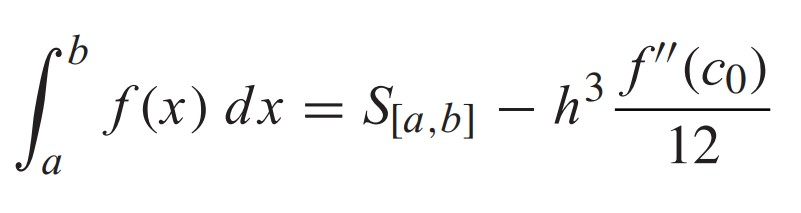
\includegraphics[scale=0.4, center]{adapt.jpg}
Untuk setiap pencarian kriterianya, akan didapatkan S[a,c]+S[c,b] dengan a<c<b pada interval [a,b] yang mengaproksimasi S[a,b]. Pengecekan dapat dilakukan antara S[a,b]-(S[a,c]+S[c,b]) hingga memenuhi kriteria 3*TOL.

3. \emph{Romberg Method}



Dalam paper ini, penulis diberikan sebuah fungsi probabilitas suatu variabel acak Z dengan distribusi normal kurang dari \emph{z} dengan fungsi integral berikut

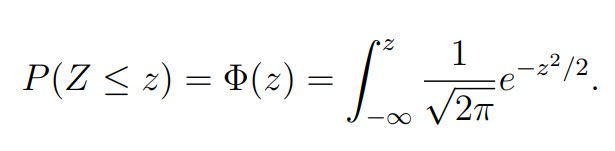
\includegraphics[scale=0.6, center]{func2.jpg}

Tujuan dari penelitian ini adalah untuk membuktikan aproksimasi nilai integral pada interval \([a, b]\) dengan ketiga metode di atas untuk menghitung probabilitas P(a kecil Z kecil B) memiliki error (perbandingan dengan nilai aktual) kurang dari \emph{TOL} yang diberikan.

\section{Implementasi Metode Composite Simpson}

\section{Implementasi Metode Adaptive Method}
Perhitungan probabilitas yang diminta adalah untuk nilai P(a<=Z<=b), sedangkan fungsi yang tersedia adalah P(Z<=z). Nilai P(a<=Z<=b) dapat diubah menyesuaikan bentuk persamaan di atas dengan cara sebagai berikut:  
P(a<=Z<=b) = F(b) - F(a)
Berdasarkan PDF, F(x) = 


\section{Implementasi Metode Romberg}


\section{Kesimpulan}
Kesimpulan disini.

% % Example of a table from http://www.latextemplates.com/template/professional-table

\begin{thebibliography}{1}
	% Here are a few examples of different citations 
	% Book
	\bibitem{kopka_1999} % Note the label in the curly brackets. Use the cite the source; e.g., \cite{kopka_latex}
	H.~Kopka and P.~W. Daly, \emph{A Guide to \LaTeX}, 3rd~ed.\hskip 1em plus
	0.5em minus 0.4em\relax Harlow, England: Addison-Wesley, 1999.
	\bibitem{horowitz_2005}D.~Horowitz, \emph{End of Time}. New York, NY, USA: Encounter Books, 2005. [E-book] Available: Ebrary, \url{http://site.ebrary.com/lib/sait/Doc?id=10080005}. Accessed on: Oct. 8, 2008.

	% Article from database
	\bibitem{castlevecchi_2008}D.~Castelvecchi, ``Nanoparticles Conspire with Free Radicals'' \emph{Science News}, vol.174, no. 6, p. 9, September 13, 2008. [Full Text]. Available: Proquest, \url{http://proquest.umi.com/pqdweb?index=52&did=1557231641&SrchMode=1&sid=3&Fmt=3&VInst=PROD&VType=PQD&RQT=309&VName=PQD&TS=1229451226&clientId=533}. Accessed on: Aug.~3, 2014.
	% Conference Paper from the Internet
	\bibitem{lach_2010}J.~Lach, ``SBFS: Steganography based file system,'' in \emph{Proceedings of the 2008 1st International Conference on Information Technology, IT 2008, 19-21 May 2008, Gdansk, Poland.} Available: IEEE Xplore, \url{http://www.ieee.org}. [Accessed: 10 Sept. 2010].
	% Web page, no author
	\bibitem{a_laymans_explanation}``A `layman's' explanation of Ultra Narrow Band technology,'' Oct.~3, 2003. [Online]. Available: \url{http://www.vmsk.org/Layman.pdf}. [Accessed: Dec.~3, 2003].
\end{thebibliography}

% This is a hand-made bibliography. If you want to use a BibTeX file, you're on your own ;-)














\end{document}